\section{Aplicación en desarrollo de aplicaciones Web} 

Como aplicaciones para los casos de prueba hemos elegido una aplicación para cada una de las tecnologías más representativas en el desarrollo web a largo de estos años:
\begin{itemize}
    \item Java
    \item PHP
    \item JavaScript
\end{itemize}	

Las aplicaciones que analizaremos serán las siguientes:

\begin{table}[htb]
    \begin{center}
      \begin{tabular}{c|c}
        \hline
        \rowcolor{tema!10} 
        \bft{Aplicación} & \bft{Tecnologías utilizadas}\\
        \hline
        \href{https://dvwa.co.uk/}{Damn Vulnerable Web application (dwva)} & PHP\\ 
        \href{https://github.com/bkimminich/juice-shop}{Juice Shop} & JavaScript, Angular, Node.js\\
        \href{https://github.com/WebGoat/WebGoat}{WebGoat} &  Java, Spring Boot  
      \end{tabular}
      \caption{Parámetros línea comandos dependency-check}
      \label{tab:tabla 2}
    \end{center}
  \end{table}
\newpage

\subsubsection{WebGoat}
Siguiendo las tareas del documento de plan pruebas para este proyecto, realizamos las tareas que se detallan a continuación.\\

Para ejecutar el análisis de dependencias desde Maven, debemos añadir la siguiente configuración del plugin de Dependency-Check:

\begin{listing}[h]
    \inputminted{xml}{./Ficheros/ConfiguracionPlugin_Maven.xml}
    \caption{Configuración plugin Dependency-Check}
    \label{listing:4}
\end{listing}

A parte de la configuración anterior debemos añadir las siguientes propiedades:\\

\begin{listing}[h]
    \inputminted{xml}{./Ficheros/ConfigPropertiesPlugin_maven.xml}
    \caption{Propiedades plugin Dependency-Check}
    \label{listing:5}
\end{listing}

Para ejecutar el escáner\\

\begin{verbatim}
    mvn dependency-check:check
\end{verbatim}

\newpage
La ejecución del análisis estático de código, así como el análisis de dependencias, lo realizaremos a través de un 
\href{https://github.com/M0l1n3ta/PFG/blob/master/Scripts/STAT/RunSonarScaner_WebGoat.ps1}{script}, con el cual
obtenemos el siguiente resultado:\\

\begin{figure}[htb] 
    \captionsetup{width=1\linewidth}   
    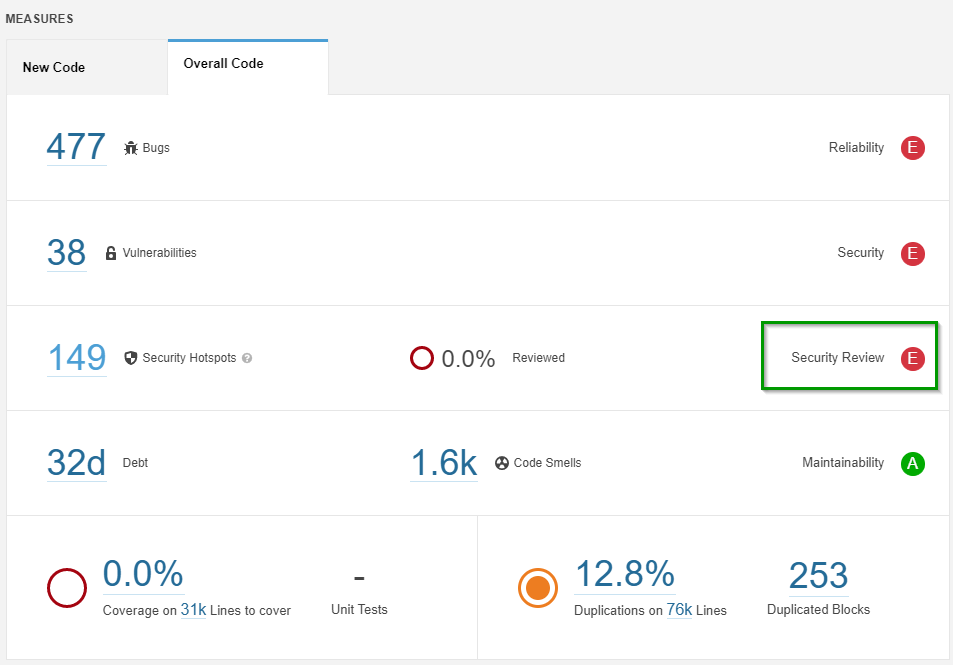
\includegraphics[width=\linewidth]{./imagenes/09_AnalisisEstatico_WebGoat.png}
    \caption{Resultado análisis estatico código WebGoat}  
    \label{fig:25}
\end{figure}

Como era de esperar obtiene el peor resultado posible en la medida de seguridad \textbf{“E”}\\

Todos los detalles de cada una de las vulnerabilidades, así como los \textbf{“hotspot”} están detalladas en el reporte de 
\href{https://github.com/M0l1n3ta/PFG/blob/master/Reportes/An%C3%A1lisis estatico de c%C3%B3digo/ReporteAnalisisestatico_WebGoat.docx}{análisis estático de código}.\\

Con los defectos encontrados con el análisis estático más la información que el pentester recolecte sobre la aplicación analizada 
se procede a crear un \href{https://github.com/M0l1n3ta/PFG/blob/master/Scripts/Plan Pruebas/PlanPruebas_OWASP_WebGoat.ps1}{plan de prueba} para la aplicación para poder capturar los hallazgos en la herramienta de análisis 
dinámico (OWASP ZAP).\\

\newpage
Antes de ejecutar el plan de pruebas levantamos la aplicación levantando el docker compose incluido en las fuentes del proyecto, para ello ejecutamos el comando:

\begin{verbatim}
    docker-compose up
\end{verbatim}

\begin{figure}[!htb]
    \captionsetup{width=1\linewidth}  
    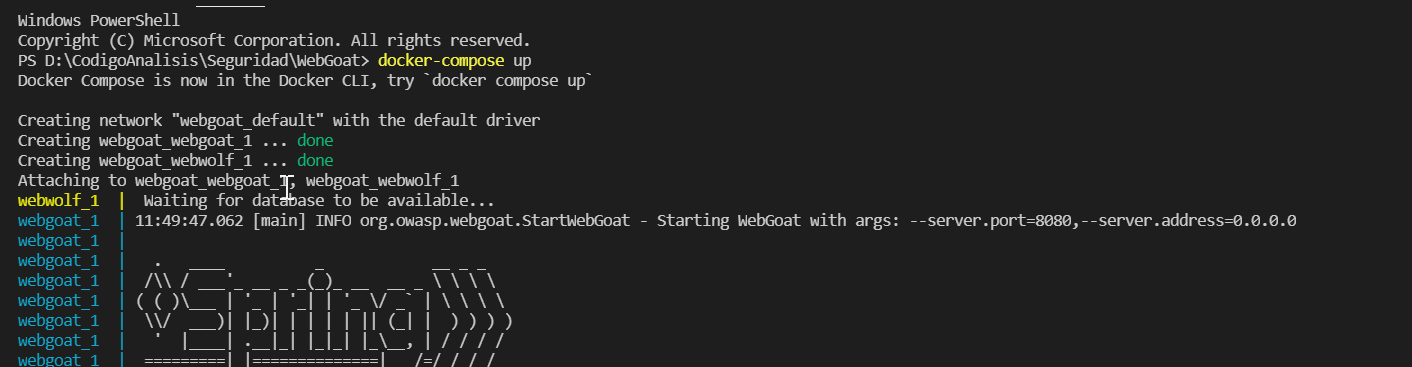
\includegraphics[width=\linewidth]{./imagenes/04_1_1_00_WebGoat_DockerComposeUP.png}
    \caption{WebGoat run docker compose}  
\end{figure}

Una vez levantada la aplicación verificamos que funciona accediendo a la \href{http://localhost:8080/WebGoat}{ruta} (\url{http://localhost:8080/WebGoat})

\begin{figure}[!htb]
    \centering
    \captionsetup{width=1\linewidth}  
    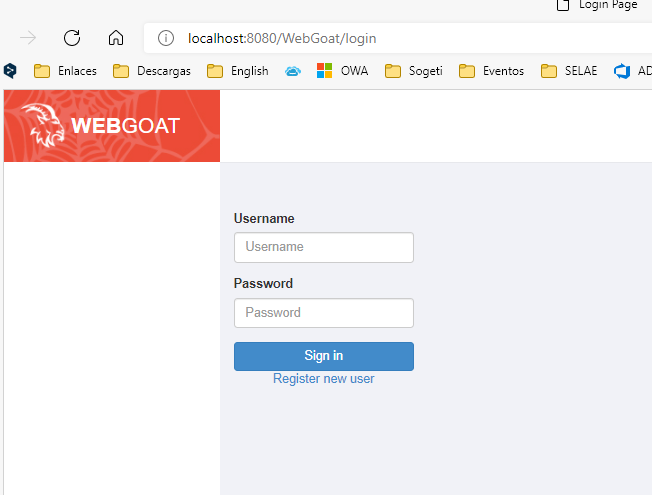
\includegraphics[width=0.8\linewidth]{./imagenes/04_1_1_01_WebGoat_APPRunning.png}
    \caption{WebGoat run docker compose}  
\end{figure}

\newpage

Una vez verificado, lanzamos el script de pruebas y revisamos que se vayan capturando la peticiones en OWASP ZAP correctamente

\begin{figure}[!htb]
    \captionsetup{width=1\linewidth}  
    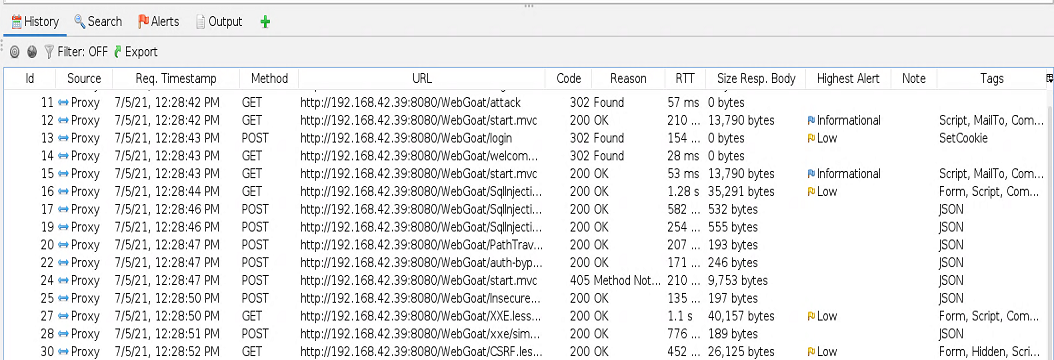
\includegraphics[width=\linewidth]{./imagenes/04_1_1_02_WebGoat_ZapProxyRQST.png}
    \caption{WebGoat Zap Proxy Requests}  
    \label{fig:WebGoat Zap Proxy Requests}
\end{figure}

Una vez finalizado el plan de pruebas lanzamos el spider para que descubra nuevas rutas en la aplicación. Una vez finalizado 
el proceso de Spider veremos la nuevas url que ha detectado, en este caso 28:\\

\begin{figure}[!htb]
    \captionsetup{width=1\linewidth}  
    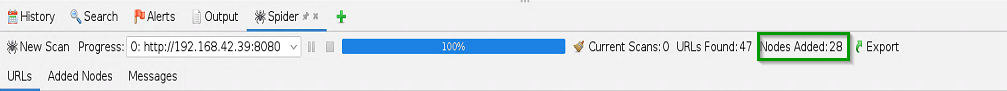
\includegraphics[width=\linewidth]{./imagenes/04_1_1_03_WebGoat_ZapProxySpiderResult.png}
    \caption{WebGoat Spider Result}  
    \label{fig:WebGoat Spider Result}
\end{figure}

\newpage
Una vez finalizado el escáner en la ventana de progreso\\
\begin{figure}[!htb]
    \centering
    \captionsetup{width=1\linewidth}  
    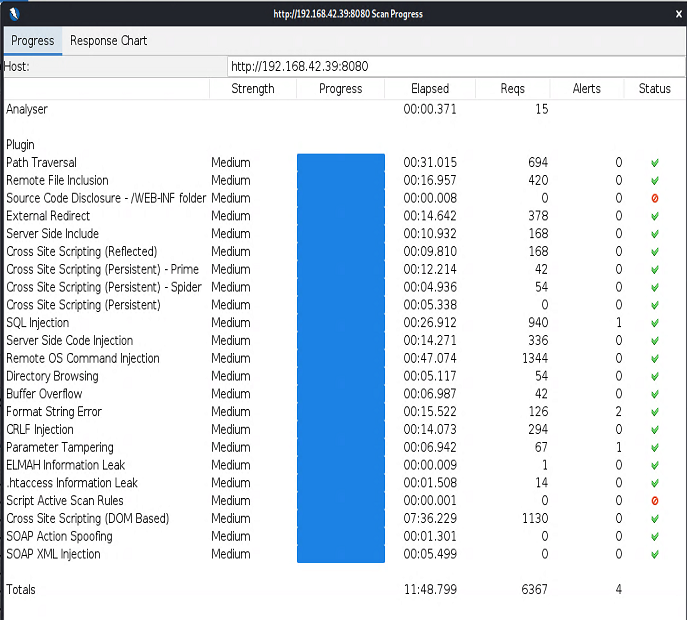
\includegraphics[scale=0.8]{./imagenes/04_1_1_04_WebGoat_ZapProxyActiveScanResult.png}
    \caption{WebGoat Active Scan Finished}  
    \label{fig:WebGoat Active Scan Finished}
\end{figure}

Podremos ver las incidencias que ha detectado en análisis dinámico de la aplicación:\\

\begin{figure}[!htb]
    \centering
    \captionsetup{width=1\linewidth}
    \begin{center}
        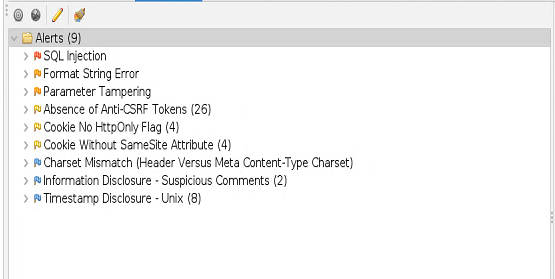
\includegraphics[scale=0.8]{./imagenes/04_1_1_05_WebGoat_ZapProxyActiveScanAlert.png}
    \end{center}  
    \caption{WebGoat Active Scan Alerts}  
    \label{fig:WebGoat Active Scan Alerts}
\end{figure}

\newpage

\subsubsection{Damn Vulnerable Web application (DVWA)}
Siguiendo las tareas del \href{https://github.com/M0l1n3ta/PFG/blob/master/Reportes/DVWA/PPR DVWA - Plan Pruebas de Seguridad.docx}{documento de plan pruebas}
para este proyecto, realizamos las tareas que se detallan a continuación.\\

Para este proyecto no se realizará análisis de dependencias puesto que el proyecto no hace uso del componente de PHP 
necesario para realizar este tipo de análisis en proyectos PHP (\href{https://getcomposer.org/}{Composer})\\

La ejecución del análisis estático de código lo realizaremos a través de un
\href{https://github.com/M0l1n3ta/PFG/blob/master/Scripts/STAT/RunSonarScaner_DWVA.ps1}{script}, con el cual obtenemos 
el siguiente resultado:\\

\begin{figure}[!htb]  
    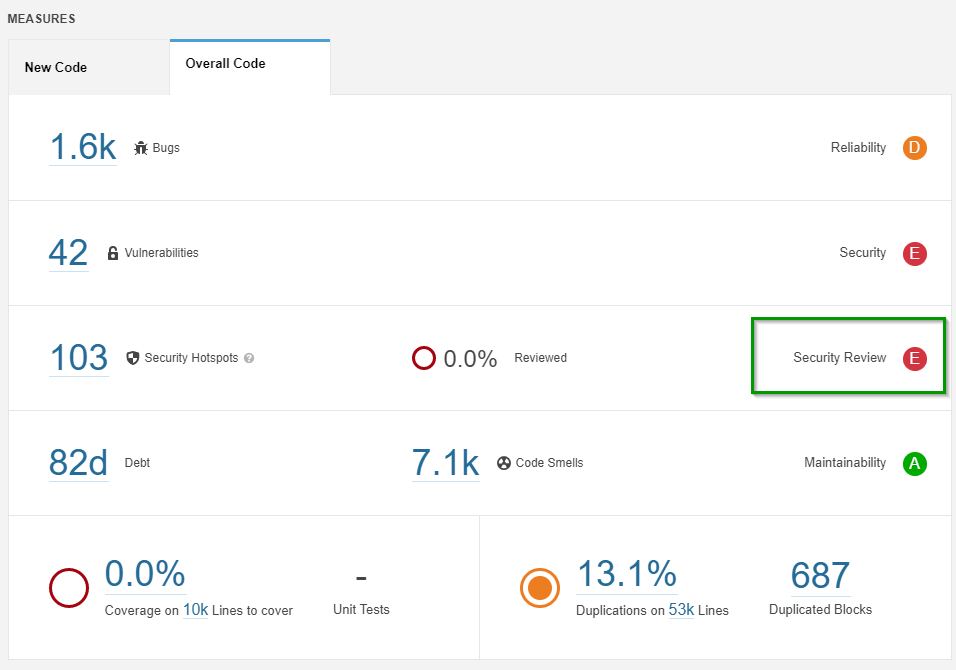
\includegraphics[width=\linewidth]{./imagenes/07_AnalisisEstatico__DVWA.png}
    \caption{Resultado análisis estatico código DVWA}  
    \label{fig:22}
\end{figure}
Como era de esperar obtiene el peor resultado posible en la medida de seguridad \textbf{“E”}

\newpage
En el apartado de \textbf{“Security hot spots”} vemos que se detectan la mayoría de las 
vulnerabilidades recogidas en el OWASP top 10:

\begin{figure}[!htb]
    \captionsetup{width=1\linewidth}  
    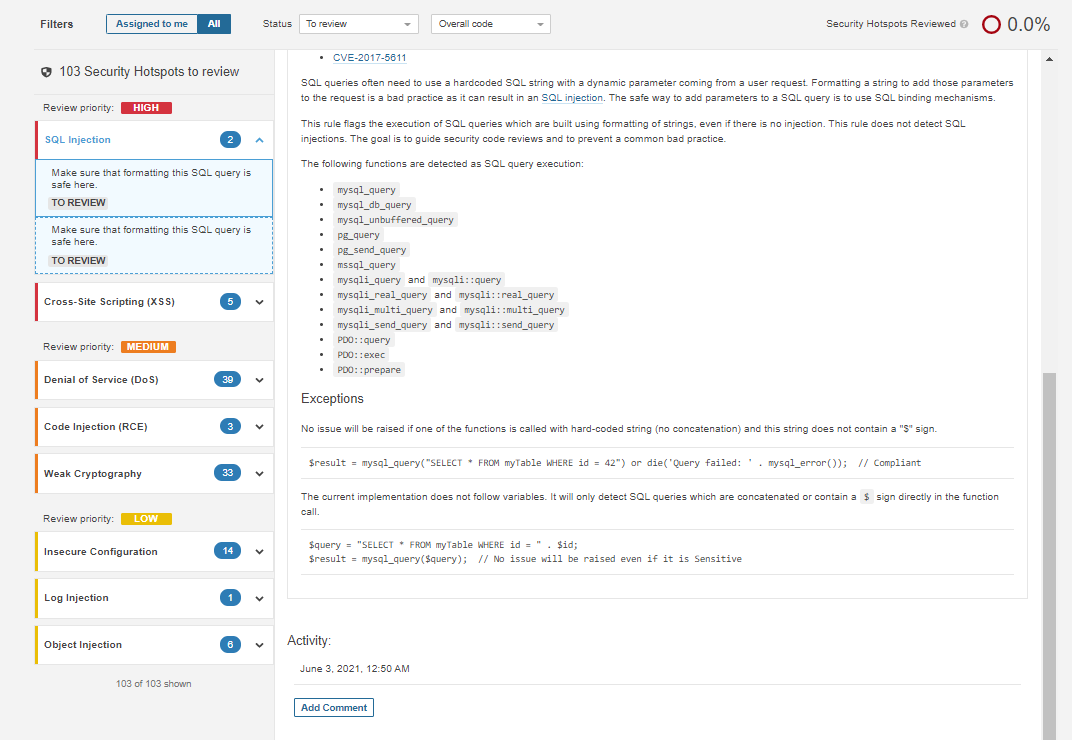
\includegraphics[width=\linewidth]{./imagenes/04_1_2_01_DVWA_Securityhotspots.png}
    \caption{DVWA Security hotspot}  
    \label{fig:DVWA Security hotspot}
\end{figure}

Todos los detalles de cada una de las vulnerabilidades, así como los \textbf{“hotspot”} están detalladas en el reporte 
de \href{https://github.com/M0l1n3ta/PFG/blob/master/Reportes/An%C3%A1lisis estatico de c%C3%B3digo/ReporteAnalisisestatico_dvwa.docx}{análisis estático de código}.\\

Con los defectos encontrados con el análisis estático más la información que el pentester vaya recolectando sobre la aplicación
analizada se procede a crear un \href{https://github.com/M0l1n3ta/PFG/blob/master/Scripts/Plan Pruebas/PlanPruebas_DVWA.ps1}{plan de prueba}
para la aplicación para poder capturar los hallazgos en la herramienta de análisis dinámico (OWASP ZAP).

\newpage
Antes de ejecutar el plan de pruebas levantamos la aplicación levantando compilando el \href{https://github.com/M0l1n3ta/PFG/blob/master/EntornoPruebas/dvwa/dockerfile}{contenedor} 
incluido en las fuentes de este PFG, puesto que el proyecto original no lo incluye, o ejecutándolo compilado desde Docker Hub 
con el siguiente comando:

\begin{verbatim}
    docker run --rm -it -p 8086:80 molineta/dvwa:2.0.1
\end{verbatim}

Una vez ejecutado verificamos que el contenedor se encuentra funcionando, accediendo a la siguiente 
ruta \url{http://localhost:8086/login.php}\\

\begin{figure}[!htb]
    \captionsetup{width=1\linewidth}  
    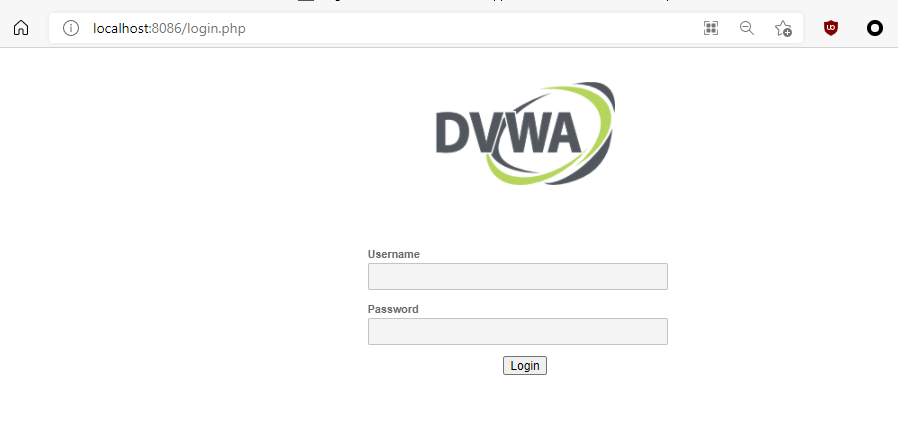
\includegraphics[width=\linewidth]{./imagenes/04_1_2_01_DVWA_ContainerUP.png}
    \caption{DVWA Application running}  
    \label{fig:DVWA Application running}
\end{figure}
Una vez verificado, lanzamos el script de pruebas y revisamos que se vayan capturando la peticiones en OWASP ZAP correctamente

\begin{figure}[!htb]
    \captionsetup{width=1\linewidth}  
    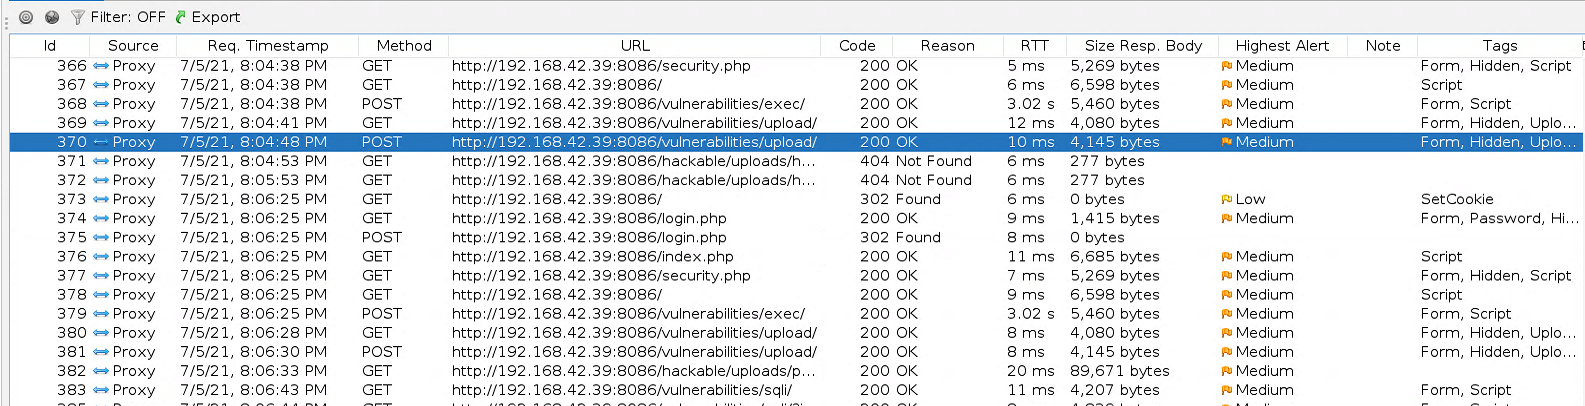
\includegraphics[width=\linewidth]{./imagenes/04_1_2_02_DVWA_ZapProxyRQST.png}
    \caption{DVWA Zap Proxy Requests}  
    \label{fig:DVWA Zap Proxy Requests}
\end{figure}

Una vez finalizado el plan de pruebas lanzamos el spider para que descubra nuevas rutas en la aplicación. Una vez finalizado
el proceso de Spider veremos la nuevas url que ha detectado, en este caso 81:

\begin{figure}[!htb]
    \captionsetup{width=1\linewidth}  
    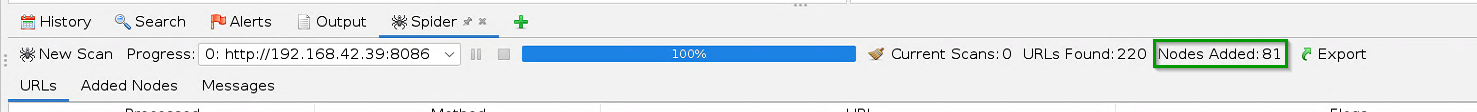
\includegraphics[width=\linewidth]{./imagenes/04_1_2_03_DVWA_ZapProxySpiderResult.png}
    \caption{WebGoat Spider Result}  
    \label{fig:DVWA Spider Result}
\end{figure}

Con la url añadidas desde el plan de pruebas, más la detectadas con el proceso de \textbf{“Spider”}, más la que el pentester
considere añadir lanzamos el proceso de análisis dinámico de código con  la política \textbf{“Default Policy”} y esperamos
que termine para ver las incidencias que ha detectado en análisis dinámico de la aplicación:

\begin{figure}[!htb]
    \captionsetup{width=1\linewidth}  
    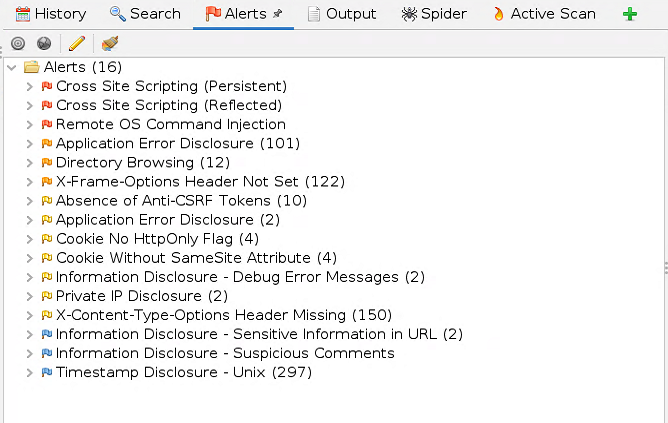
\includegraphics[width=\linewidth]{./imagenes/04_1_2_04_DVWA_ZapProxyActivescanAlerts.png}
    \caption{DVWA Active Scan Alerts}  
    \label{fig:DVWA Active Scan Alerts}
\end{figure}

\newpage

\subsubsection{Juice Shop}
Siguiendo las tareas del documento de plan pruebas para este proyecto, realizamos las tareas que se detallan a continuación.\\

La ejecución del análisis estático de código, así como el análisis de dependencias, lo realizaremos a través de un 
\href{https://github.com/M0l1n3ta/PFG/blob/master/Scripts/STAT/RunSonarScaner_JuiceShop.ps1}{script}, con el cual obtenemos 
el siguiente resultado:\\

\begin{figure}[!htb]
    \centering  
    \captionsetup{width=1\linewidth}  
    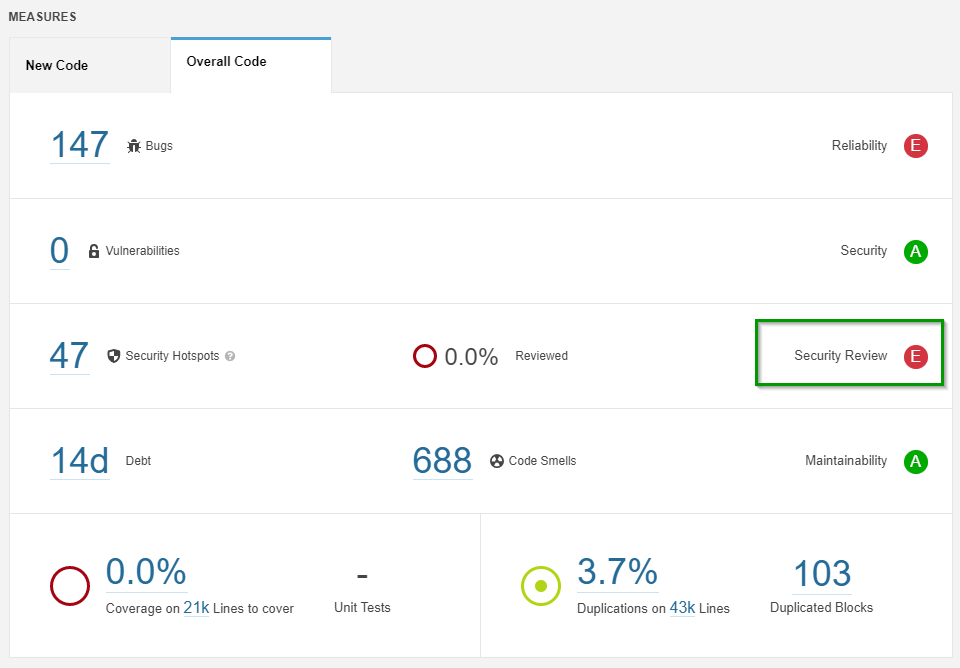
\includegraphics[width=\linewidth]{./imagenes/08_AnalisisEstatico_JuiceShop.png}
    \caption{Resultado análisis estatico código Juice Shop}  
    \label{fig:23}
\end{figure}

Como era de esperar obtiene el peor resultado posible en la medida de seguridad \textbf{“E”}

Todos los detalles de cada una de las vulnerabilidades, así como los \textbf{“hotspot”} están detalladas en el reporte de 
\href{https://github.com/M0l1n3ta/PFG/blob/master/Reportes/An%C3%A1lisis estatico de c%C3%B3digo/ReporteAnalisisestatico_JuiceShop.docx}{análisis estático de código}.

Con los defectos encontrados con el análisis estático más la información que el pentester vaya recolectando sobre la aplicación 
analizada se procede a crear un \href{https://github.com/M0l1n3ta/PFG/blob/master/Scripts/Plan Pruebas/PlanPruebas_OWASP_JuiceShop.ps1}{plan de prueba} 
para la aplicación para poder capturar los hallazgos en la herramienta de análisis dinámico (OWASP ZAP).

\newpage

Antes de ejecutar el plan de pruebas levantamos la aplicación compilando el contenedor incluido en las fuentes 
del proyecto o ejecutándolo compilado desde Docker Hub con el siguiente comando:

\begin{verbatim}
    docker run --rm -it -p 3000:3000 molineta/juiceshop:12.7.2
\end{verbatim}

Una vez ejecutado verificamos que el contenedor se encuentra funcionando, accediendo a la siguiente 
ruta \url{http://localhost:3000}

\begin{figure}[!htb]
    \captionsetup{width=1\linewidth}  
    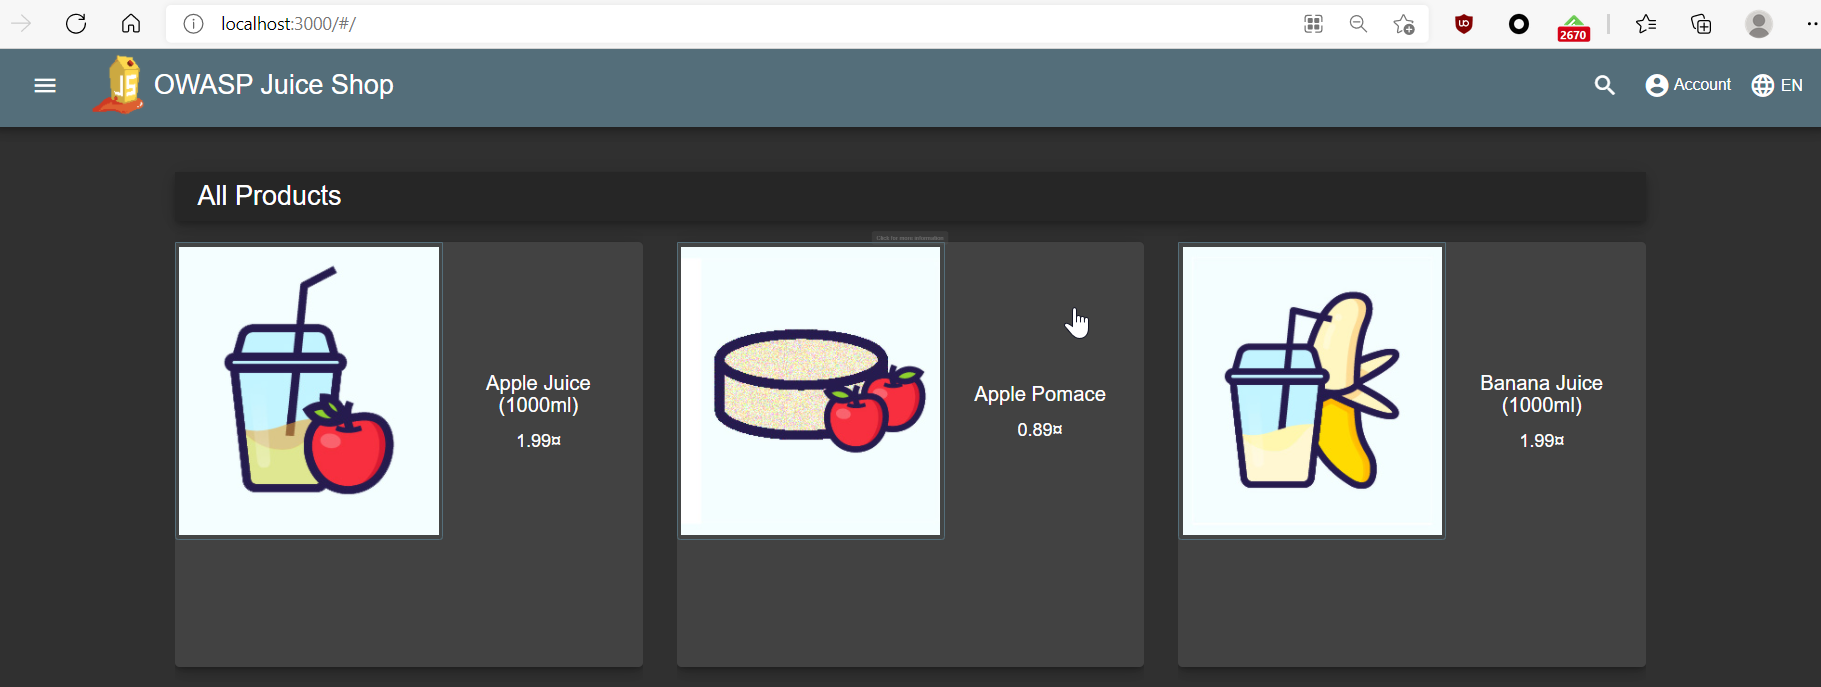
\includegraphics[width=\linewidth]{./imagenes/04_1_3_01_JuiceShop_ContainerUP.png}
    \caption{JuiceShop Application running}  
    \label{fig:JuiceShop Application running}
\end{figure}

Una vez verificado, lanzamos el script de pruebas y revisamos que se vayan capturando la peticiones en OWASP ZAP correctamente\\
\begin{figure}[!htb]
    \captionsetup{width=1\linewidth}  
    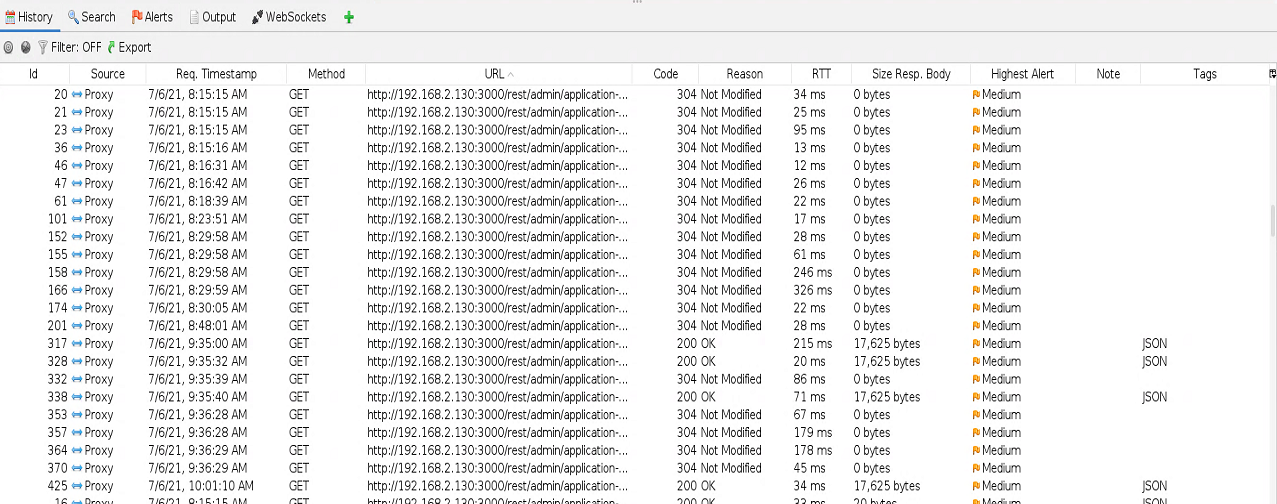
\includegraphics[width=\linewidth]{./imagenes/04_1_3_02_JuiceShop_ZapProxyRQST.png}
    \caption{JuiceShop Zap Proxy Requests}  
    \label{fig:JuiceShop Zap Proxy Requests}
\end{figure}

Una vez finalizado el plan de pruebas lanzamos el spider para que descubra nuevas rutas en la aplicación. Una vez finalizado 
el proceso de Spider veremos la nuevas url que ha detectado, en este caso 288:\\

\begin{figure}[!htb]
    \captionsetup{width=1\linewidth}  
    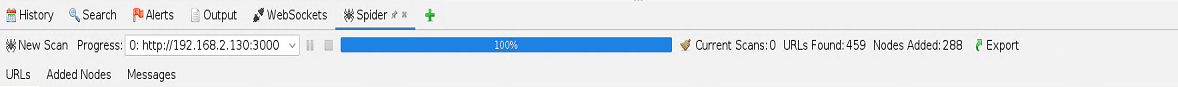
\includegraphics[width=\linewidth]{./imagenes/04_1_3_03_JuiceShop_ZapProxySpiderResult.png}
    \caption{JuiceShop Spider Result}  
    \label{fig:JuiceShop Spider Result}
\end{figure}

Con la url añadidas desde el plan de pruebas, más la detectadas con el proceso de \textbf{“Spider”}, más la que el pentester 
considere añadir lanzamos el proceso de análisis dinámico de código con  la política \textbf{“Default Policy”} y esperamos
que termine para ver las incidencias que ha detectado en análisis dinámico de la aplicación:\\

\begin{figure}[!htb]
    \captionsetup{width=1\linewidth}  
    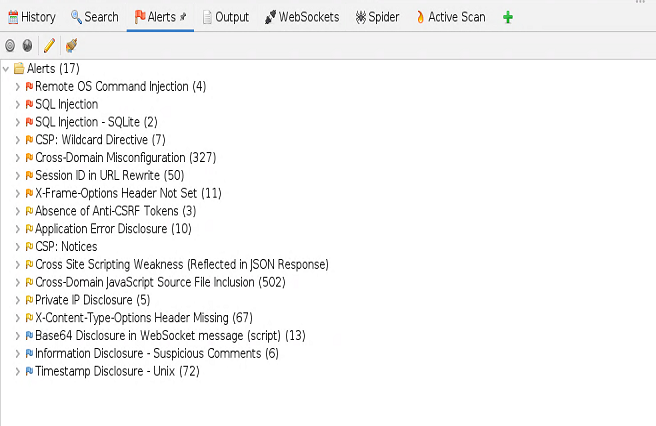
\includegraphics[width=\linewidth]{./imagenes/04_1_3_04_JuiceShop_ZapProxyActiveScanResult.png}
    \caption{JuiceShop Active Scan Alerts}  
    \label{fig:JuiceShop Active Scan Alerts}
\end{figure}
